% !TeX TXS-program:compile = txs:///pdflatex/[--shell-escape]
\chapter{Decomposition into periodic characters}
\label{ch:Analysis}
%% ==============================

As our goal is to represent general dynamic networks and temporal graphs as EPGs, one problem is the missing periodicity in general temporal and dynamic graphs. 

\begin{figure}[h]
	\begin{minipage}[t]{0.49\textwidth}
		\centering
		\begin{tikzpicture}[every edge quotes/.style = {auto, font=\footnotesize, sloped}]
			\begin{scope}[every node/.style={circle,fill}]
				\node (A) at (0,0) {};
				\node (B) at (0,2) {};
				\node (C) at (2,0) {};
				\node (D) at (2,2) {};
				\node (E) at (1,3) {};
			\end{scope}
			
			\draw (A) edge["101\dots"] (B)
			(B) edge["100\dots"] (C)
			(D) edge["001\dots"] (C)
			(A) edge["000\dots"] (C)
			(D) edge["111\dots"] (E)
			(B) edge["011\dots"] (D)
			(B) edge["101\dots"] (E);	
		\end{tikzpicture}
	\end{minipage}
	\begin{minipage}[t]{0.49\textwidth}
		\centering
		\begin{tikzpicture}[every edge quotes/.style = {auto, font=\footnotesize, sloped}]
			\begin{scope}[every node/.style={circle,fill}]
				\node (A) at (0,0) {};
				\node (B) at (0,2) {};
				\node (C) at (2,0) {};
				\node (D) at (2,2) {};
				\node (E) at (1,3) {};
			\end{scope}
			
			\draw (A) edge["101"] (B)
			(B) edge["100"] (C)
			(D) edge["0010"] (C)
			(A) edge["0"] (C)
			(D) edge["110"] (E)
			(B) edge["01111"] (D)
			(B) edge["10"] (E);
		\end{tikzpicture}
	\end{minipage}
	\caption{TODO}
\end{figure}

\section{Decomposing the edge labels}

Initially, we start with a temporal graph where all edge labels $\tau(e)$ have fixed length and there are no periods present. To find and analyze such periods in the given labels, the algorithm from \cite{DBLP:journals/corr/abs-2107-04683} is used and adapted to our problem. To apply the algorithm which is defined for automata, a label $ w \in \{0,1\}^*$ is interpreted as an unary automata. In the label either the $0s$ or the $1s$ symbols are used to represent final states $Q_f$. The algorithm from \cite{DBLP:journals/corr/abs-2107-04683} can be simplified due to the fact that we only represent unary automata and therefore only have a single transition from each state, basically forming a simple circle of all possible states. Using the fact that our alphabet is of size one, $|\Sigma| = 1$ we only need to follow a single transition and furthermore, we do not need to check each state separately, we only need to check multiples of the chosen period. This means that for a period length of $i$ we only have to check $i$ states on the circle being in the same state. We also only need to check up to factors of the length of the label $n$ since they cover all states and periods. The factors are tested one by one in an ascending manner, so that small periods will cover states first. This also implies that the larges possible period, which will only cover a single state, is considered a trivial period and covering a label with only trivial periods is always possible.


\begin{figure}
	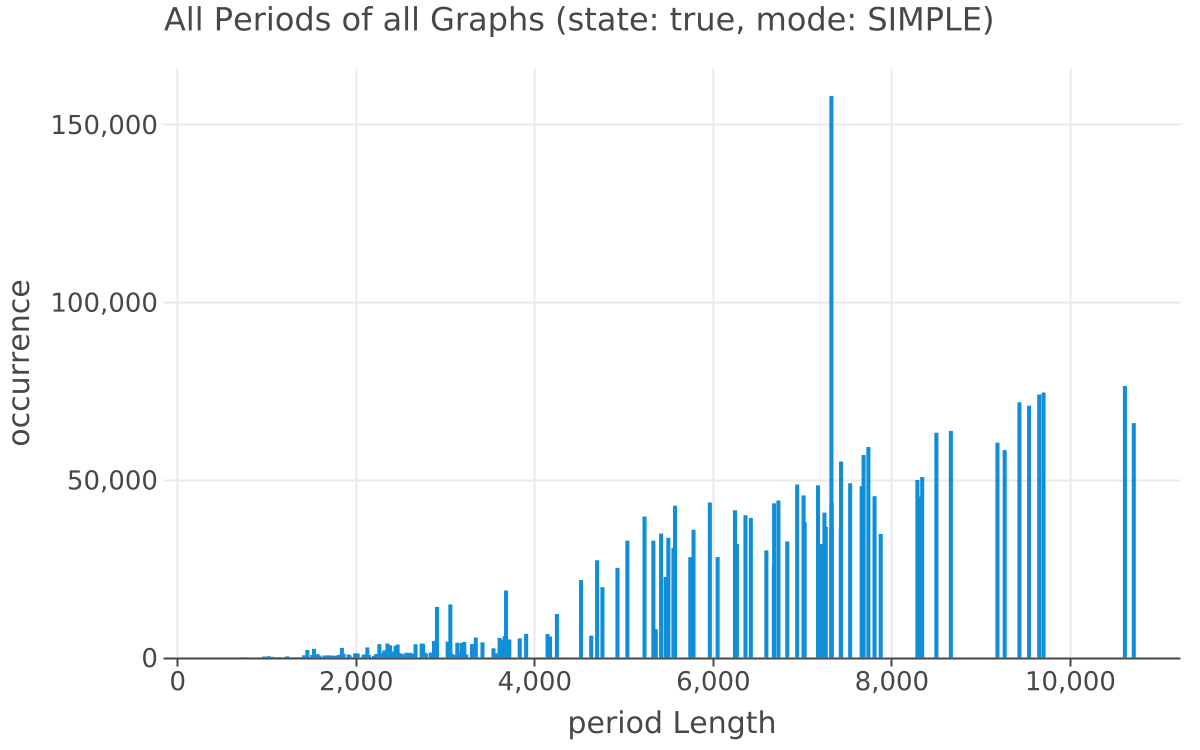
\includegraphics[width=\linewidth]{plots/all-graphs-bar-char-strue-mSIMPLE.png}
	\caption{A subfigure}
	\label{fig:sub1}
\end{figure}

\begin{figure}
	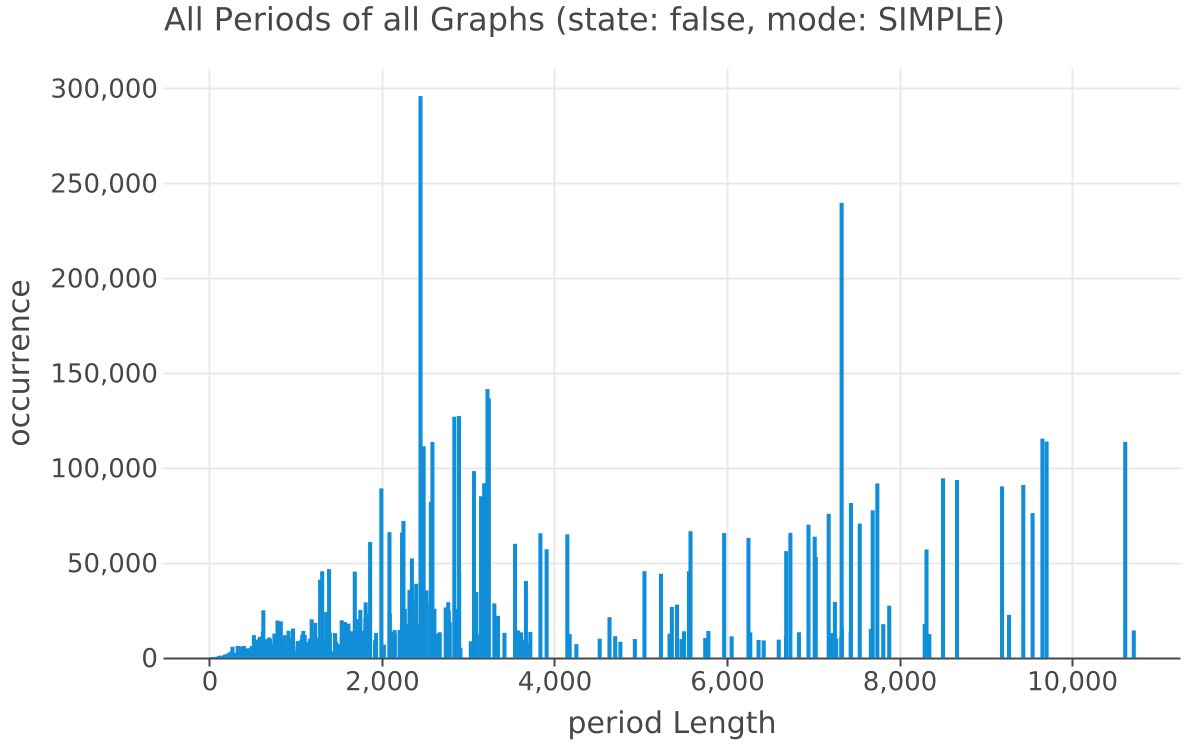
\includegraphics[width=\linewidth]{plots/all-graphs-bar-char-sfalse-mSIMPLE.png}
	\caption{A subfigure}
	\label{fig:sub1}
\end{figure}



\begin{figure}
	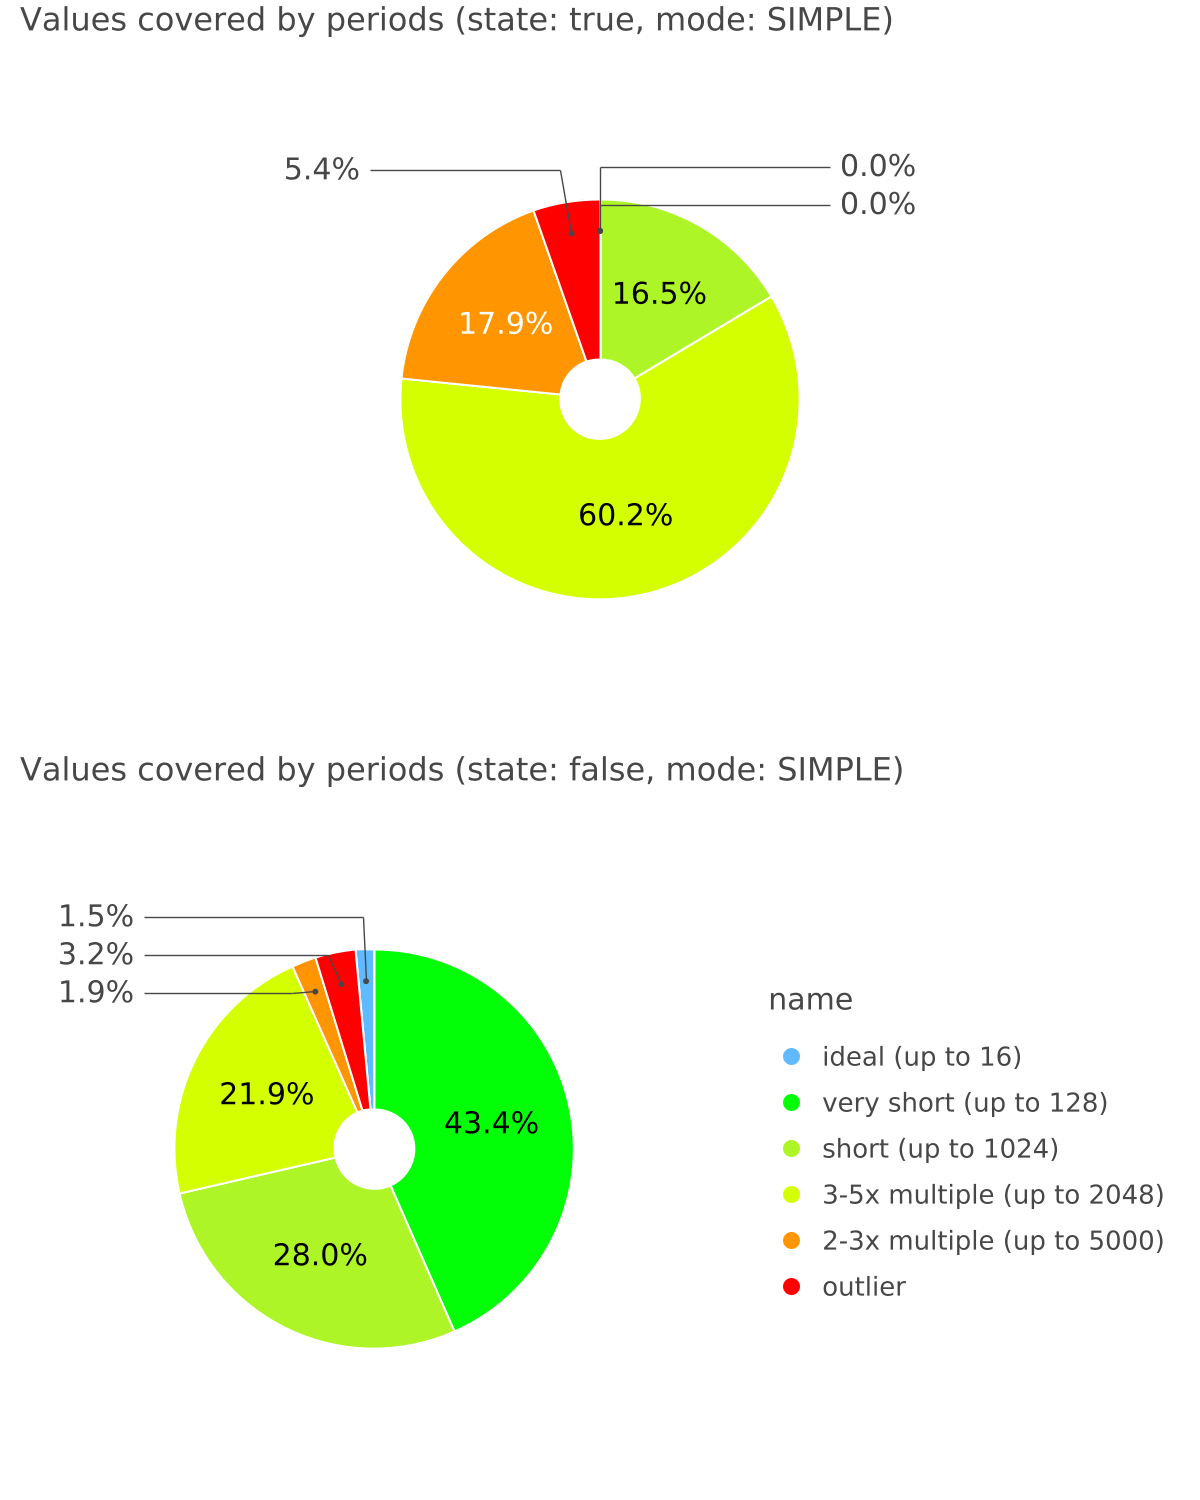
\includegraphics[width=\linewidth]{plots/all-covered-values-pie-chart-combined-ontop.png}
	\caption{A subfigure}
	\label{fig:sub2}
\end{figure}



\section{Combining periods into a periodic edge label}

Now with the collection of periods, novel problems arises. How to combine the periods in the most optimal manner? What is the minimal number of periods needed to cover a given array? These and other questions where tried to answer both theoretically and empirically with some real world data.

